\newcommand{\packedTagResultsAucTable}{
    \begin{table}[H]
        \centering
        \begin{tabular}{|p{2,8cm}||p{2,8cm} p{2,8cm} p{2,8cm}|}
            \hline
            Packed Tag & ALOHA & Joint Embedding & Proposed Model \\
            \hline
            AUC-ROC & 0.513$\pm$0.007 & 0.513$\pm$0.009 & \textBF{0.539$\pm$0.003} \\
            \hline
        \end{tabular}
        \caption{AUC-ROC (Area Under Curve) of the different models for the \textbf{Packed Tag} prediction task. Results were aggregated over \textBF{3} training runs with different weight initializations and minibatch orderings. Best results are shown in \textbf{bold}.} \label{tab:packedTag_auc}
    \end{table}
}

\newcommand{\packedTagResultsAtFprTable}{
    \begin{center}
        \begin{longtable}[c]{|p{3,2cm}||p{1,8cm} p{1,8cm} p{1,8cm} p{1,8cm} p{1,8cm}|}
            \hline
            Packed Tag & \multicolumn{5}{c|}{{FPR}} \\
            & $10^{-5}$ & $10^{-4}$ & $10^{-3}$ & $10^{-2}$ & $10^{-1}$ \\
            \hline
            \endfirsthead

            \caption*{\raggedright ...continued from previous page} \\
            \hline
            Packed Tag & \multicolumn{5}{c|}{\textbf{FPR}} \\
            & $10^{-5}$ & $10^{-4}$ & $10^{-3}$ & $10^{-2}$ & $10^{-1}$ \\
            \hline
            \endhead

            \caption*{\raggedleft ...continued on next page} \\
            \endfoot

            \caption{Mean and standard deviation results (TPR, Accuracy, Recall, Precision and F1-Score) of the different models for the \textbf{Packed Tag} prediction task at different \textbf{FPR}s (\textit{False Positive Rates}). Results were aggregated over \textBF{3} training runs with different weight initializations and minibatch orderings. Best results are shown in \textbf{bold}. Under \textbf{TPR} results are also presented the percentage reduction in mean detection error and in ROC curve standard deviation introduced by the \textit{Proposed Model} with respect to both \textit{ALOHA} model and \textit{Joint Embedding}.} \label{tab:packedTag_results_at_fpr} \\
            \endlastfoot

            \multicolumn{6}{|c|}{\textbf{TPR}} \\
            \hline
            ALOHA & \textBF{0.002$\pm$0.002} & \textBF{0.002$\pm$0.002} & \textBF{0.003$\pm$0.003} & 0.008$\pm$0.004 & 0.110$\pm$0.015 \\
            Joint Embedding & \textBF{0.002$\pm$0.002} & \textBF{0.002$\pm$0.002} & 0.002$\pm$0.002 & \textBF{0.014$\pm$0.003} & \textBF{0.125$\pm$0.007} \\
            Proposed Model & 0.000$\pm$0.000 & 0.000$\pm$0.000 & 0.000$\pm$0.000 & 0.011$\pm$0.002 & 0.113$\pm$0.004 \\
            \hline
            Error Reduction wrt \newline ALOHA & -0.2\% & -0.2\% & -0.3\% & 0.3\% & 0.3\% \\
            Error Reduction wrt \newline Joint Embedding & -0.2\% & -0.2\% & -0.2\% & -0.3\% & -1.4\% \\
            \hline
            Std Reduction wrt \newline ALOHA & 100.0\% & 100.0\% & 100.0\% & 50.0\% & 73.3\% \\
            Std Reduction wrt \newline Joint Embedding & 100.0\% & 100.0\% & 100.0\% & 33.3\% & 42.9\% \\
            \hline
            \multicolumn{6}{|c|}{\textbf{Accuracy}} \\
            \hline
            ALOHA & \textBF{0.882$\pm$0.000} & \textBF{0.882$\pm$0.000} & \textBF{0.881$\pm$0.000} & \textBF{0.875$\pm$0.001} & 0.807$\pm$0.002 \\
            Joint Embedding & \textBF{0.882$\pm$0.000} & \textBF{0.882$\pm$0.000} & \textBF{0.881$\pm$0.000} & \textBF{0.875$\pm$0.001} & \textBF{0.809$\pm$0.000} \\
            Proposed Model & 0.881$\pm$0.000 & 0.881$\pm$0.000 & \textBF{0.881$\pm$0.000} & 0.874$\pm$0.000 & 0.807$\pm$0.000 \\
            \hline
            \multicolumn{6}{|c|}{\textbf{Recall}} \\
            \hline
            ALOHA & \textBF{0.002$\pm$0.002} & \textBF{0.002$\pm$0.002} & \textBF{0.003$\pm$0.003} & 0.008$\pm$0.004 & 0.110$\pm$0.015 \\
            Joint Embedding & \textBF{0.002$\pm$0.002} & \textBF{0.002$\pm$0.002} & 0.002$\pm$0.002 & \textBF{0.014$\pm$0.003} & \textBF{0.125$\pm$0.007} \\
            Proposed Model & 0.000$\pm$0.000 & 0.000$\pm$0.000 & 0.000$\pm$0.000 & 0.011$\pm$0.002 & 0.113$\pm$0.004 \\
            \hline
            \multicolumn{6}{|c|}{\textbf{Precision}} \\
            \hline
            ALOHA & \textBF{1.000$\pm$0.000} & \textBF{1.000$\pm$0.000} & \textBF{0.500$\pm$0.408} & 0.113$\pm$0.053 & 0.130$\pm$0.016 \\
            Joint Embedding & \textBF{1.000$\pm$0.000} & \textBF{1.000$\pm$0.000} & 0.333$\pm$0.236 & \textBF{0.167$\pm$0.018} & \textBF{0.145$\pm$0.006} \\
            Proposed Model & \textBF{1.000$\pm$0.000} & \textBF{1.000$\pm$0.000} & 0.000$\pm$0.000 & 0.131$\pm$0.016 & 0.132$\pm$0.004 \\
            \hline
            \multicolumn{6}{|c|}{\textbf{F1 Score}} \\
            \hline
            ALOHA & \textBF{0.005$\pm$0.003} & \textBF{0.005$\pm$0.003} & \textBF{0.007$\pm$0.006} & 0.015$\pm$0.008 & 0.119$\pm$0.015 \\
            Joint Embedding & \textBF{0.005$\pm$0.003} & \textBF{0.005$\pm$0.003} & 0.005$\pm$0.003 & \textBF{0.025$\pm$0.005} & \textBF{0.134$\pm$0.006} \\
            Proposed Model & 0.000$\pm$0.000 & 0.000$\pm$0.000 & 0.000$\pm$0.000 & 0.021$\pm$0.003 & 0.122$\pm$0.004 \\
            \hline
        \end{longtable}
    \end{center}
}

\newcommand{\packedTagResultsSummaryTable}{
    \begin{table}[H]
        \centering
        \begin{tabular}{|p{3,2cm}||p{1,8cm} p{1,8cm} p{1,8cm} p{1,8cm} p{1,8cm}|}
            \hline
            \multicolumn{6}{|c|}{Packed Tag (at FPR $=1\%$)} \\
            \hline
            Model & TPR & Accuracy & Precision & Recall & F1 score \\
            \hline
            ALOHA & 0.008$\pm$0.004 & \textBF{0.875$\pm$0.001} & 0.113$\pm$0.053 & 0.008$\pm$0.004 & 0.015$\pm$0.008 \\
            Joint Embedding & \textBF{0.014$\pm$0.003} & \textBF{0.875$\pm$0.001} & \textBF{0.167$\pm$0.018} & \textBF{0.014$\pm$0.003} & \textBF{0.025$\pm$0.005} \\
            Proposed Model & 0.011$\pm$0.002 & 0.874$\pm$0.000 & 0.131$\pm$0.016 & 0.011$\pm$0.002 & 0.021$\pm$0.003 \\
            \hline
        \end{tabular}
        \caption{Summary of the mean and standard deviation results of the different models for the \textbf{Packed Tag} prediction task at \textbf{FPR} $=1\%$. Results were aggregated over \textBF{3} training runs with different weight initializations and minibatch orderings. Best results are shown in \textbf{bold}.} \label{tab:packedTag_result_summary}
    \end{table}
}

\newcommand{\packedTagRocAloha}{
    \begin{figure}[H]
        \vspace*{-0.5cm}
        \centering
        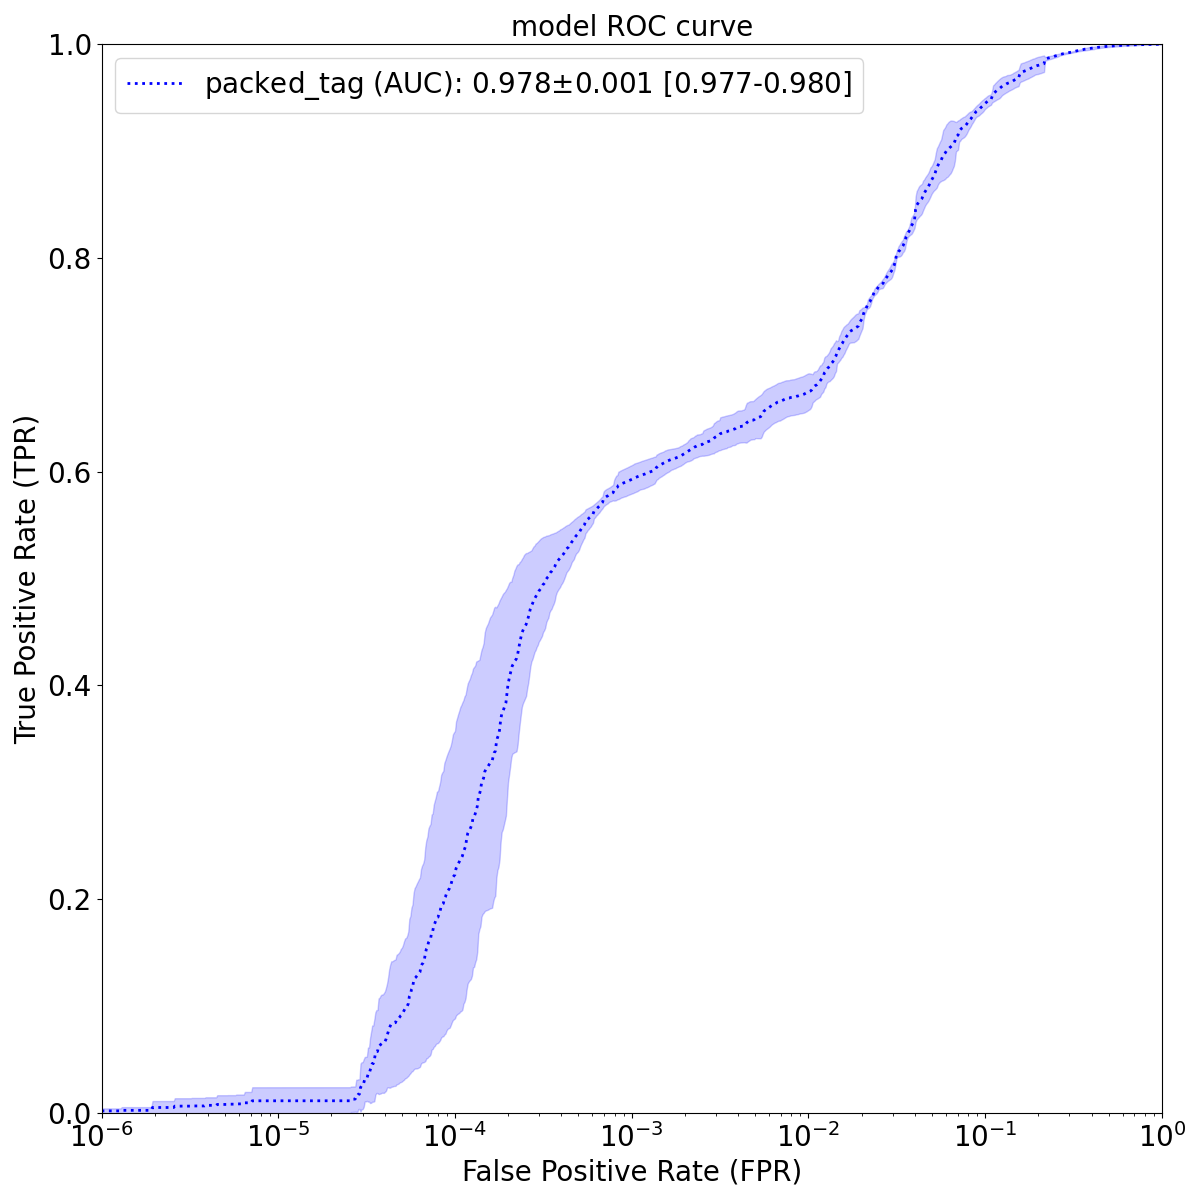
\includegraphics[width=0.6\textwidth]{./results/packed_tag_roc_aloha.png}
        \vspace*{-0.2cm}
        \caption{ROC curve and AUC statistics of \textBF{ALOHA} model for the \textbf{Packed Tag}. The line represents the \textit{mean} TPR at a given FPR, while the shaded region represents the \textit{standard deviation}. Statistics were computed over \textBF{3} training runs, each with random parameter initialization.}
        \label{fig:packedTagRocAloha}
    \end{figure}
}

\newcommand{\packedTagRocJointEmbedding}{
    \begin{figure}[H]
        \vspace*{-0.5cm}
        \centering
        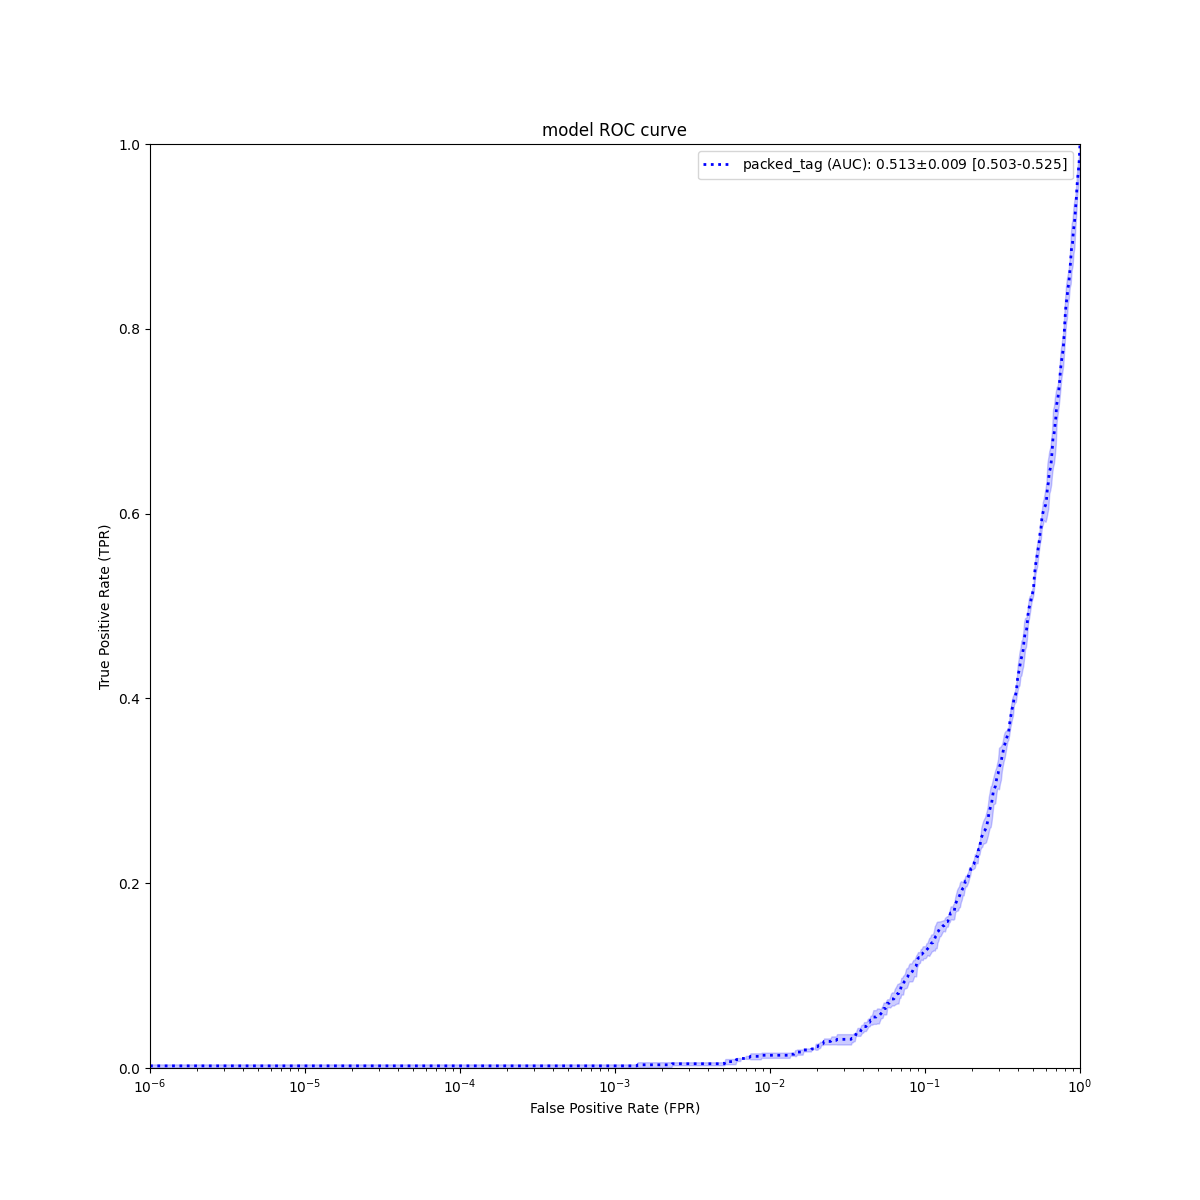
\includegraphics[width=0.6\textwidth]{./results/packed_tag_roc_jointEmbedding.png}
        \vspace*{-0.2cm}
        \caption{ROC curve and AUC statistics of \textBF{Joint Embedding} model for the \textbf{Packed Tag}. The line represents the \textit{mean} TPR at a given FPR, while the shaded region represents the \textit{standard deviation}. Statistics were computed over \textBF{3} training runs, each with random parameter initialization.}
        \label{fig:packedTagRocJointEmbedding}
    \end{figure}
}

\newcommand{\packedTagRocProposedMethod}{
    \begin{figure}[H]
        \vspace*{-0.5cm}
        \centering
        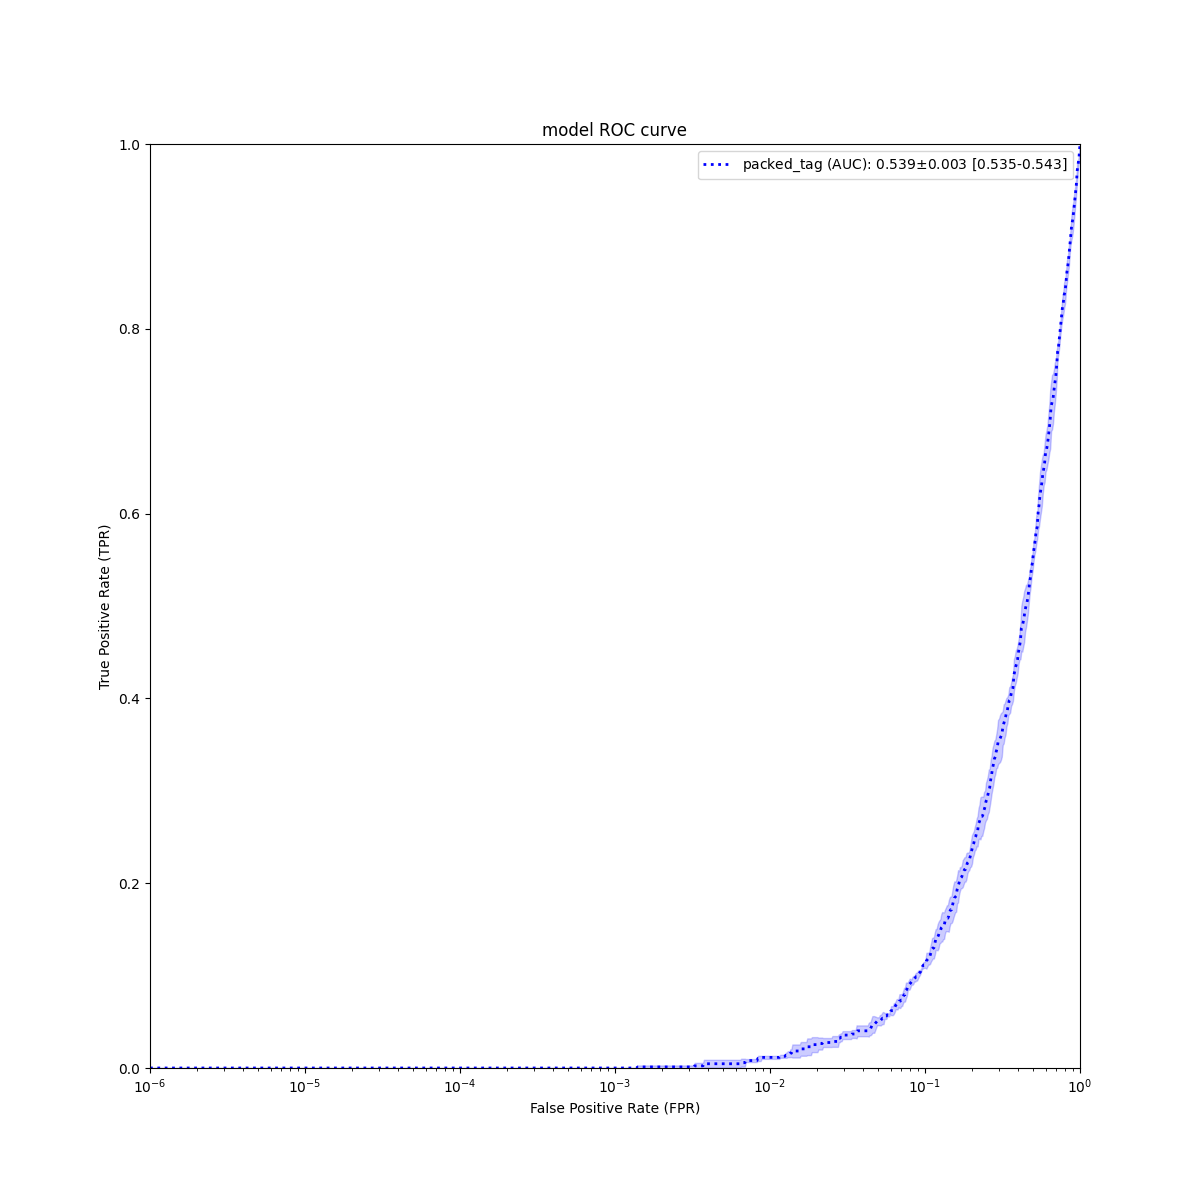
\includegraphics[width=0.6\textwidth]{./results/packed_tag_roc_proposedModel.png}
        \vspace*{-0.2cm}
        \caption{ROC curve and AUC statistics of \textBF{Proposed Model} for the \textbf{Packed Tag}. The line represents the \textit{mean} TPR at a given FPR, while the shaded region represents the \textit{standard deviation}. Statistics were computed over \textBF{3} training runs, each with random parameter initialization.}
        \label{fig:packedTagRocProposedModel}
    \end{figure}
}
